\section{Réglementation aéronautique}
	\subsection{Les organisations}
		\subsubsection{L'OACI}
		
		\begin{wrapfigure}{l}{0.45\textwidth}
		
\includegraphics[width=0.9\linewidth]{02-Navigation/img/OACI-logo.pdf} 
		\legende{Logo de l'OACI}{img:OACI-logo}
		\end{wrapfigure}
		
		L'\acrshort{oaci} (\acrlong{oaci} \anglais{International Civil Aviation Organization, ICAO}) a été fondée en 1944 par la convention de Chicago, son siège est à Montréal (Canada). Elle regroupe la majorité des états du monde (192 en 2025, dont tous les pays d'Europe\footnote{hors Vatican et le Liechtenstein}). \\
		
		L'OACI établit des \textbf{normes} et des \textbf{pratiques recommandées}. Ces normes et recommandations concernant tous les domaines de l'aéronautique civile : licences, cartes, aérodromes, exploitation et gestion de la navigabilité des aéronefs, télécommunications, enquêtes sur les accidents et incidents aériens...
		
		\info{Les codes uniques attribués à chaque aérodrome (par exemple LFBD pour Bordeaux Mérignac) sont également appelés "code OACI". Il s'agit d'un exemple concret de l'application d'une norme OACI.}
		
		\subsubsection{L'EASA}
		
		\begin{wrapfigure}{r}{0.45\textwidth}
		
\includegraphics[width=0.9\linewidth]{02-Navigation/img/EASA-logo.pdf} 
		\legende{Logo de l'OACI}{img:EASA-logo}
		\end{wrapfigure}
		
		L'\acrshort{easa} (\anglais{\acrlong{easa} - Agence de l'Union européenne pour la sécurité aérienne}) est une agence de l'Union Européenne qui traite de la sécurité aérienne et créée en 2003. \\
		
		Initialement l'EASA œuvrait essentiellement sur la certification des aéronefs. Ses missions se sont ensuite étendues à l'exploitation des aéronefs, les licences des personnels navigants (ce qui permet aux pilotes formés en Europe d'exercer leurs fonctions dans tous les pays de l'Union Européenne sans "conversion" de licence).
		
		\subsubsection{La DGAC}
		\begin{wrapfigure}{l}{0.4\textwidth}
		
\includegraphics[width=0.9\linewidth]{02-Navigation/img/DGAC-logo.pdf} 
		\legende{Logo de la DGAC}{img:DGAC-logo}
		\end{wrapfigure}
		La \acrshort{dgac} (\acrlong{dgac}) l'administration française qui regroupe l'ensemble des services de l'État chargés de réglementer et de superviser la sécurité aérienne, le transport aérien et les activités de l'aviation civile en général.
		
		Cette administration gère notamment :
		\begin{itemize}
		  \item le contrôle aérien sur le territoire français,
		  \item la certification des aéronefs et la gestion de la navigabilité des aéronefs immatriculés en France.
	    \end{itemize}
		
		Acteur de la prévention, la DGAC a pour mission de veiller non seulement à la sécurité et au bien-être des hommes mais aussi à la préservation de l'environnement, en luttant contre les nuisances dues au transport aérien.
			
	
	\subsection{L'organisation de l'espace aérien}
	Afin de permettre aux aéronefs d'évoluer en toute sécurité, l'espace aérien a été divisé en différents espaces, qui présentent chacun des conditions d'accès spécifiques et des services associés.
		
		\subsubsection{Les classes d'espaces aériens}
		Au niveau mondial, l'OACI a défini 7 \glspl{classe d'espace aérien}, nommées par des lettres de A (classe présentant le plus de contraintes) à G (classe présentant le moins de contraintes). Dans ce chapitre, nous allons voir quelles sont les différences entre ces classes.
		
		La connaissance des règles qui régissent les espaces aérien est primordiale car les pilotes doivent impérativement avoir conscience à chaque instant du service qu'ils peuvent attendre des services de contrôle avec lequel ils sont en contact.\\
		
		Les espaces peuvent-être actifs en permanence ou seulement à certains horaires. Quand ils ne sont pas actifs, les espaces sont généralement déclassés en espace de classe G. Les horaires d'activation se trouvent dans l'\acrshort{aip}. \\
		
		On peut subdiviser ces 7 espaces en 2 sous groupes : \textbf{les espaces contrôlés} (de A à E) et \textbf{les espaces non contrôlés} (F et G). \\
		
		Selon la classe d'espace ou l'on se trouve, les services rendus diffèrent. Voici les principaux services qui peuvent être rendus :
		\begin{itemize}
			\item Contrôle - séparation de trafic : avec ce service, c'est au contrôle que revient la charge de séparer les différents aéronefs pour éviter tout risque de collision. Pour cela, le contrôleur dispose généralement de radars qui lui permettent de localiser précisément les différents appareils sous sa responsabilité
			\item Contrôle - information de circulation : avec ce service, le contrôleur informe les commandants de bord de la présence d'autres aéronefs. C'est ensuite aux commandants de bord d'assurer la séparation (généralement visuelle) à partir des informations communiquées par le contrôle
			\item Information et alerte : ce service consiste pour le contrôle à fournir des informations de position des aéronefs dont le contrôleur à connaissance. A la demande des pilotes, le contrôle peut également fournir des informations météorologiques, des informations sur les aérodromes ou encore fournir de l'aide (et déclencher les secours) en cas de situation de détresse.
		\end{itemize}
		
		\paragraph{Espaces contrôlés}
		Dans les espaces contrôlés, le contact radio est obligatoire (avec une exception pour les vols VFR en classe E), et la pénétration est soumise à une \textbf{clearance} du contrôleur. Ces espaces sont placés sous l'autorité d'un contrôleur aérien, qui est chargé d'assurer l'efficacité et la sécurité du trafic dans sa zone.
		
		Dans ces espaces, les conditions météorologiques de vol à vue (\acrshort{vmc}) sont :
		\begin{itemize}
		\item distance par rapport aux nuages : 1500 mètres horizontalement et 300 mètres (1000 ft) verticalement ;
		\item visibilité 8 km au-dessus du FL 100 et 5 km au-dessous du FL 100. 
		\end{itemize}
		
		\subparagraph{Classe A}
		Cette classe d'espace est interdite aux VFR. Seuls les vols IFR y sont admis et le contrôle assure la séparation entre ces vols.
		
		\info{En France, les seules classes A se trouvent en région parisienne.}
		
		La vitesse n'y est pas limitée (grâce à la séparation garantie par le contrôle).
		
		\subparagraph{Classe B}
		Tous les types de vol (IFR et VFR) sont autorisés en espace de classe B. Le contrôle assure la séparation de tous les aéronefs.
		
		\info{Cette classe d'espace n'existe pas en France.}
		
		La vitesse n'y est pas limitée (grâce à la séparation garantie par le contrôle).
		
		\subparagraph{Classe C}
		Tous les types de vol (IFR et VFR) sont autorisés en espace de classe C. Le contrôle assure :
		\begin{itemize}
		\item la séparation entre les vols IFR,
		\item la séparation entre les vols IFR et les vols VFR,
		\item l'information de trafic entre les vols VFR
		\end{itemize}
		
		\info{En France cette classe est utilisée essentiellement pour les TMA.}
		
		La vitesse est limitée à 250 kt pour les VFR sous le niveau de vol 100, sauf autorisation du contrôle.
		
		\subparagraph{Classe D}\label{classeD}
		Tous les types de vol (IFR et VFR) sont autorisés en espace de classe D. Le contrôle assure :
		\begin{itemize}
		\item la séparation entre les vols IFR,
		\item la séparation entre les vols IFR et VFR spécial,
		\item l'information de trafic entre les vols IFR et les vols VFR,
		\item l'information de trafic entre les vols VFR
		\end{itemize}
		
		\info{En France cette classe est utilisée essentiellement pour les CTR.}
		
		La vitesse est limitée à 250 kt pour tous les vols sous le niveau de vol 100, sauf autorisation du contrôle.
		
		\subparagraph{Classe E}
		Tous les types de vol (IFR et VFR) sont autorisés en espace de classe E. Le contrôle assure :
		\begin{itemize}
		\item la séparation entre les vols IFR,
		\item l'information de trafic entre les vols IFR et les vols VFR, si possible,
		\item l'information de trafic entre les vols VFR, si possible
		\end{itemize}
		
		\info{En France cette classe est utilisée essentiellement pour les TMA.}
		
		\info{Les espaces de classe E ont la particularité de faire cohabiter les vols IFR qui y sont contrôlés avec les vols VFR qui n'y sont pas contrôlés. Dans ces espaces, les commandants de bord des vols VFR ne sont pas soumis à obligation de contact radio ni d'obtention de \textit{clearance}. La séparation entre les vols IFR et VFR non connus du contrôle est donc assurée essentiellement via la règle du \textit{voir et éviter}.}
		
		La vitesse est limitée à 250 kt pour tous les vols sous le niveau de vol 100, sauf autorisation du contrôle.
		
		\paragraph{Espaces non contrôlés}
		Dans ces espaces, le contact radio n'est pas obligatoire, pas plus que l'obtention de \textit{clearance}. La règle de base est donc le voir et éviter entre tous les types de vol.
				
				
		La vitesse est limitée à 250 kt pour tous les vols sous le niveau de vol 100.
		
		Les conditions VMC dans ces espaces sont les suivants :
		\begin{itemize}
			\item hors des nuages
			\item visibilité horizontale :
			\begin{itemize}
				\item 1,5 km pour une vitesse indiquée inférieur à 140 kt (800 m pour les hélicoptères)
				\item 5 km pour une vitesse indiquée supérieur à 140 kt, limitée à 250 kt
			\end{itemize}
		\end{itemize}
		
		\subparagraph{Classe F}
		Les vols IFR peuvent bénéficier d'un service consultatif qui assurera autant que possible l'espacement entre les vols IFR connus. 
		
		\info{Cette classe d'espace n'existe pas en France.}
		
		\subparagraph{Classe G}
		Les seuls services rendus dans ces espaces est le service d'information et d'alertes.
		
		\info{Il s'agit de la classe d'espace par défaut, utilisée quand aucun autre espace n'est défini. La majorité de l'espace aérien français est de classe G.}
		
		\subsubsection{Les zones à statut particulier}
			\paragraph{Les zones R}
			Les zones R sont des zones \textbf{R}estreintes. La pénétration de ces zones est possible sous condition. Par exemple, \hyperlink{ignOaciBordeaux.1}{sur la carte extrait de Bordeaux (cf \ref{ignOaciBdx} page \pageref{ignOaciBdx})}, on peut entrer dans la zone R~204~L3 si on est en contact avec le service d'information de vol Aquitaine Info\footnote{Source : extrait de l'ENR5.1 "VFR : pénétration après contact radio avec AQUITAINE INFO. Veille radio obligatoire."}.
			
			Ces zones peuvent être actives en permanence ou seulement sur certaines tranches horaire.
			
	\begin{figure}[H]
	\centering
	\begin{minipage}[c]{0.5\linewidth}
	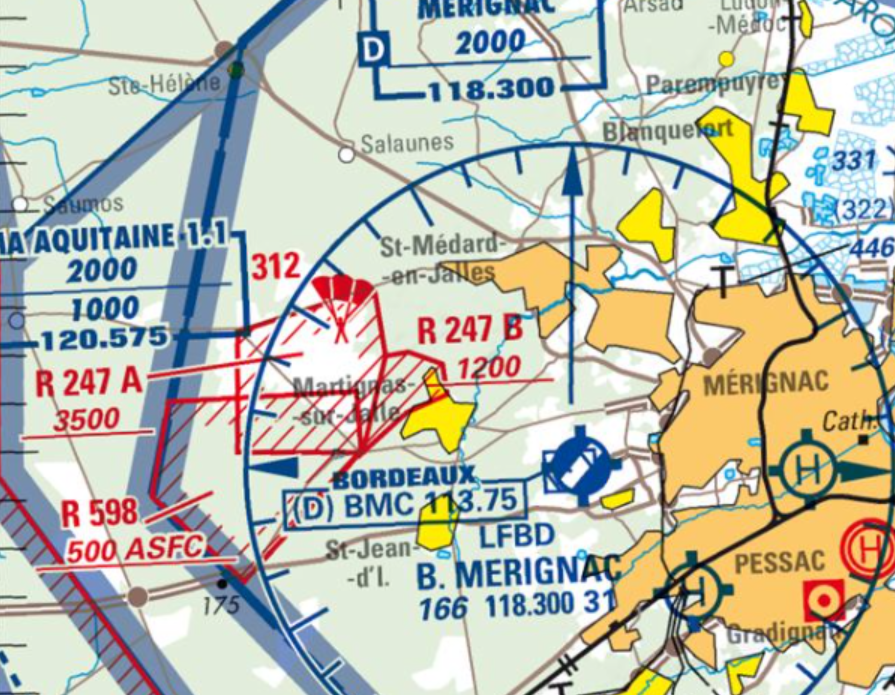
\includegraphics[width=\linewidth]{02-Navigation/img/IGN_OACI_R247_R_598.png}
	\legende{La zone restreinte R257A/B et R598}{img:ignOaci}
	\end{minipage}
	\end{figure}
			
			\paragraph{Les zones D}
			Les zone D sont des zones \textbf{D}angereuses. Leur pénétration n'est pas formellement interdite mais les activités qui s'y déroulent sont suffisamment risquées pour qu'il existe une nécessité d'avertir les navigateurs aériens. Pour ces zones, on dispose généralement d'un organisme à contacter par radio pour connaitre l'activité réelle.
			
			\alert{Il ne faut pas confondre les zones D avec les espaces aériens de classe D (cf \ref{classeD} page \pageref{classeD}).}
			
			Ces zones peuvent être actives en permanence ou seulement sur certaines tranches horaire.
			
	\begin{figure}[H]
	\centering
	\begin{minipage}[c]{0.5\linewidth}
	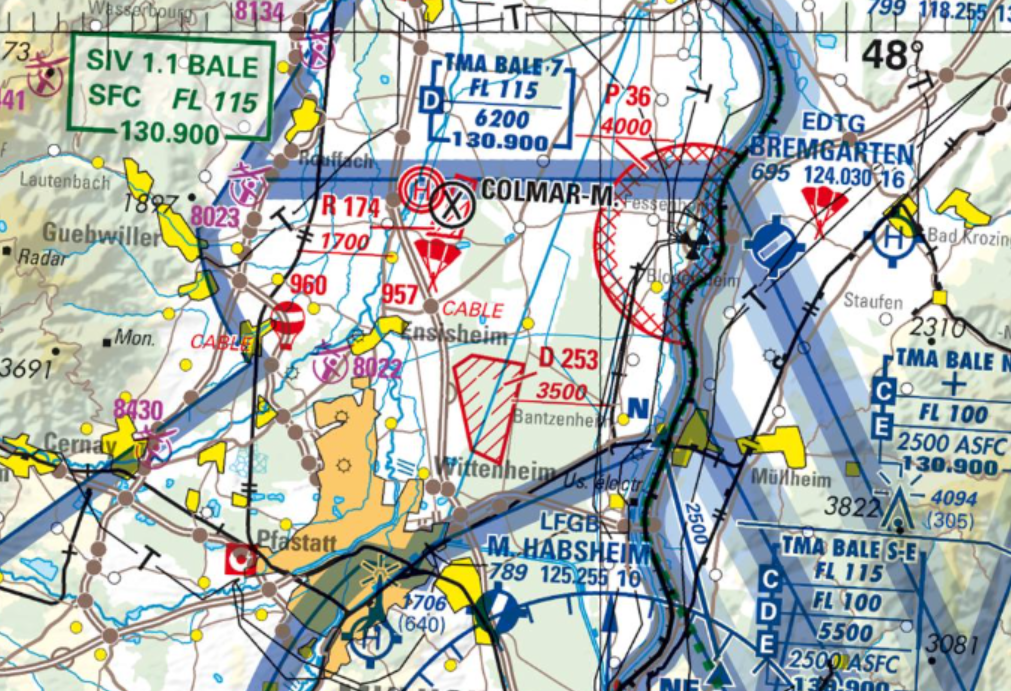
\includegraphics[width=\linewidth]{02-Navigation/img/IGN_OACI_D253.png}
	\legende{La zone dangereuse D253}{img:ignOaci}
	\end{minipage}
	\end{figure}
			
			\paragraph{Les zones P}
			Les zones P sont des zones interdites (\textbf{P}rohibées). Le vol dans ces zones est en général strictement interdit. En France, ces zones protègent généralement des infrastructures critiques, comme des centrales nucléaires. Par exemple, \hyperlink{ignOaciBordeaux.1}{sur la carte extrait de Bordeaux (cf \ref{ignOaciBdx} page \pageref{ignOaciBdx})}, la zone P~5 protège les installations du laser mégajoule au Barp. Cette zone est interdit de pénétration sauf pour les vols IFR ayant obtenu l'autorisation du contrôle, les vols de secours qui ne peuvent contourner dans le cadre de leur missions, et les aéronefs spécifiquement autorisés\footnote{Source : ENR 5.1 1.2.1}.
			
			Ces zones sont généralement actives en permanence.
			
	\begin{figure}[H]
	\begin{minipage}[c]{0.5\linewidth}
	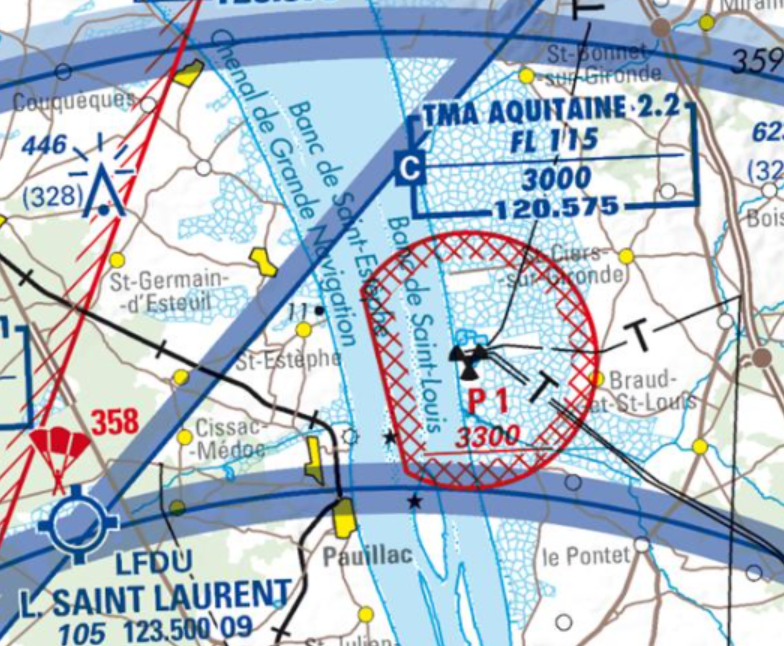
\includegraphics[width=\linewidth]{02-Navigation/img/IGN_OACI_P1.png}
	\legende{La zone interdite P1}{img:ignOaci}
	\end{minipage}
	\hfill
	\begin{minipage}[c]{0.5\linewidth}
	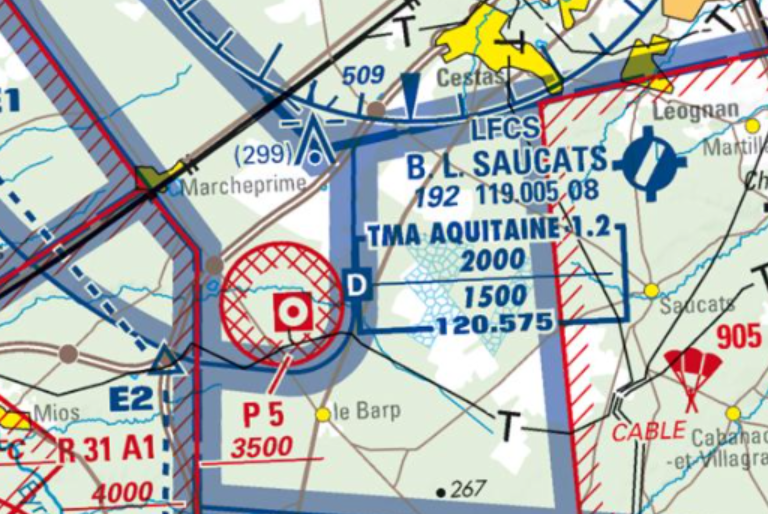
\includegraphics[width=\linewidth]{02-Navigation/img/IGN_OACI_P5.png}
	\legende{La zone interdite P5}{img:ignOaci}
	\end{minipage}
	\end{figure}
	
	\subsection{Titres aéronautiques}
	
	\subsection{Contrôle d'un aéronef}